\documentclass[12pt]{article}
\usepackage{color}
\usepackage{units}
\makeatletter
\usepackage{fullpage}
\usepackage{subcaption}
\usepackage{float}
\usepackage{amsmath}
\usepackage[dvipsnames]{xcolor}
\usepackage{url}
% \usepackage{cite}
\usepackage{nameref,hyperref}
% \usepackage[fontsize=13pt]{fontsize}
\usepackage{graphicx}
% \bibliographystyle{plain}
\usepackage{newtxtext}
\usepackage{newtxmath}
\usepackage{indentfirst}
\usepackage{setspace}
\renewcommand{\baselinestretch}{1.5}
% import Eq and Section references from the main manuscript where needed
% \usepackage{xr}
% \externaldocument{manuscript}
\usepackage{xifthen}
% define counters for reviewers and their points
\usepackage{float}

\definecolor{bl}{HTML}{005086}   %318fb5
\newcommand{\bl}[1]{{\color{bl}#1}}
\newcounter{reviewer}
\setcounter{reviewer}{0}
\newcounter{point}[reviewer]
\setcounter{point}{0}
\renewcommand{\fnum@figure}{RFig ~\thefigure}
\newcommand{\blue}[1]{{\color{blue}#1}}
% This refines the format of how the reviewer/point reference will appear.
\renewcommand{\thepoint}{P\,\thereviewer.\arabic{point}}

% command declarations for reviewer points and our responses
%\newcommand{\reviewersection}{\stepcounter{reviewer} \bigskip \hrule
%                  \section*{Reviewer \thereviewer}}
\newcommand{\reviewersection}{\stepcounter{reviewer} \bigskip
\section*{Reviewer \thereviewer}}
\newenvironment{Comment}{ \bigskip \noindent  {\textbf{[General Comment]}}  } {\par }
\newenvironment{point}{\refstepcounter{point} \bigskip \noindent {\textbf{[Reviewer~Point~\thepoint]} }  }{\par }
\newcommand{\shortpoint}[1]{\refstepcounter{point}  \bigskip \noindent
{\textbf{Reviewer~Point~\thepoint} } ---~#1\par }
\newenvironment{reply}{\medskip \noindent \textbf{Response}:\  \color{blue}\ignorespaces}{\medskip}
\newcommand{\shortreply}[2][]{\medskip \noindent
  \begin{sf}\textbf{Reply}:\  #2
    \ifthenelse{\equal{#1}{}}{}{ \hfill \footnotesize (#1)}%
    \medskip
\end{sf}}
\newcommand{\minew}[1]{{\color{red}{#1}}}
\makeatother

\begin{document}

\section*{Response to Reviewers}

\begin{flushleft}
	Dear Editor,
\end{flushleft}

On behalf of my co-authors: Yekun Zhu and Min Tang. I would like to submit the revised manuscript.

We appreciate you and the reviewers for your precious time in reviewing our paper and providing thoughtful and insightful comments.
We have addressed every comment, and believe that, taken together, the reviewers' comments have improved the manuscript significantly.
We hope that the revised manuscript now satisfies the reviewers' requirements, and hereby submit the revised manuscript for publication.
The authors welcome further constructive comments if any.

Below we provide the point-by-point responses. All modifications in the manuscript have been highlighted in \textcolor{purple}{purple}.

\begin{flushleft}
	Sincerely,

	Zheng Ma

	Shanghai Jiao Tong University
\end{flushleft}

\newpage

% Let's start point-by-point with Reviewer 1
\reviewersection{}
\begin{Comment}
	This manuscript presents DeepRTE, a novel neural operator framework designed for solving the steady-state Radiative Transfer Equation (RTE) using a physics-informed, attention-based architecture. The proposed method incorporates elements such as pre-training with delta-function boundary conditions, multi-head attention modules, and Green’s function theory. The authors claim superior efficiency and generalization capabilities, with zero-shot learning for new boundary conditions.

	While the ambition and novelty of the work are commendable, the manuscript suffers from significant issues in mathematical rigor, clarity, and the justification of design choices. Below are detailed comments and suggestions.
\end{Comment}

\begin{reply}
	We would like to thank you for your careful reading, helpful comments, and constructive suggestions, which have significantly improved the presentation of our manuscript.

	We have extensively revised the manuscript to address all the issues raised. For the mathematical rigor concerns, we have almost completely rewritten Section 2 and added numerous references to clarify the assumptions and properties of the operators and functions involved. For the design choices, we have included extensive additional numerical experiments to validate the linearity properties in Section 5.3.2 and demonstrate the design rationale and performance of each module in our architecture in Section 6.

	These changes are highlighted in \textcolor{purple}{purple} in the revised manuscript and have substantially improved the presentation of our work.

	We also want to point out that this paper primarily focuses on constructing a novel numerical algorithm using a neural network (operator) approach. While perfect mathematical rigor cannot always be achieved, we have made our best effort to make the approach as rigorous as possible. The mathematical framework presented here serves to make the neural network interpretable and guide the architectural design.

	The following are our point-by-point responses to the comments and suggestions.
\end{reply}

\begin{point}
	The mapping $A: (I_{-};\mu_t,\mu_s,p) \mapsto I$ defined in Eq. (5) and the subsequent operator decomposition are introduced without a rigorous specification of the function spaces, regularity assumptions, or operator bounds. Furthermore, the convergence of the Neumann-like expansion in Eq. (14)
	is assumed without justification. Please clearly define the function spaces (e.g., $L^1$, $L^2$, Sobolev) for $I_{-}$, $I$, and the scattering kernel $p$,and provide references or analysis to support the convergence of the series expansion. The contractive nature of the operator $LS$ should be established under well-defined assumptions.
\end{point}

\begin{reply}
	Thank you for pointing out this important issue.
	In Section 2, we have added a detailed literature review and discussion of the function spaces and assumptions for $\mu_t$, $\mu_s$, $p$ and $I_{-}$. All the main theorems used in our paper are based on the references~\cite{egger2014lp,egger2014stationary} which are now properly cited in the revised manuscript.

	Theorem 2.1~\cite{egger2014lp} provides a rigorous statement of the $L^p$ existence, uniqueness, and \emph{a priori} estimates for solutions in a more general setting where $\mu_t$, $\mu_s$, and the solution $I$ depend not only on the spatial variable $\mathbf{r}$ and angular variable $\Omega$, but also on the velocity magnitude $|\mathbf{v}|$. For the steady RTE, the velocity magnitude $|\mathbf{v}|$ can be treated as a parameter, allowing the equation to be solved for each fixed $|\mathbf{v}|$. The solution to the original problem is then obtained by integrating over $|\mathbf{v}|$ when needed. This generalization is particularly important for applications such as neutron transport, where particles exhibit a range of speeds, and radiation therapy, where frequency (related to $|\mathbf{v}|$) plays a crucial role. Extending our approach to handle velocity-dependent problems represents a promising direction for future research.

	Theorem 2.2~\cite{egger2014stationary} establishes the $L^2$ existence, uniqueness and \emph{a priori} of the solution for the steady RTE with exactly the same setting as in our algorithm and numerical experiments with mild assumptions on $\mu_t$, $\mu_s$ and $p$.

	Theorem 2.3~\cite{egger2014lp} prove the spectral radius of the operator $\mathcal{L}\mathcal{S}$ is strictly less than $1$ under the same assumptions as in Theorem 2.1 and 2.2, which guarantees the convergence of the fixed-point iteration (23) and Neumann-like expansion in (25). The contractive nature of the operator $\mathcal{L}\mathcal{S}$ in $L^1$ is also included in the reference~\cite{egger2014lp}.

	All newly added parts are highlighted in {\color{purple}purple}. Hope this addresses your concern. Thank you again for your valuable comment.
\end{reply}

\begin{point}
	The definition of the Green's function $G(r,r',\Omega,\Omega')$ in Eq. (16) is distributional in nature, involving Dirac delta functions, but it is later treated as a smooth trainable kernel in the neural network (Eq. (23)). This inconsistency raises concerns regarding the learnability and representation
	fidelity of the kernel, especially when approximating distributions with smooth networks. Clarify whether $G$ is a classical function or a distribution, and explain how the network approximates such a structure. If mollified Gaussians are used to represent boundary delta functions, discuss the convergence of this approximation and its implications on model accuracy.
\end{point}

\begin{reply}
	Thank you for your valuable comment. You are correct that the definition of Green's function in Eq. (28) is distributional in nature and may involve Dirac delta functions or singularities, as discussed in~\cite{choulli1999inverse}.

	In our neural network implementation, we do not directly learn the exact Green's function. Instead, we learn a smooth approximation $G^{\text{NN}}$ that can be effectively represented by a neural network (as in Eq. (33)). This approach is analogous to smoothed particle hydrodynamics or particle methods used in computational fluid dynamics, where singular kernels are replaced by smooth approximations~\cite{chertock2017practical}.

	We have rewrite Section 4.2 and have added detailed numerical analysis in Theorem 4.2 to discuss the convergence properties of this approximation. We also conducted extensive numerical experiments to verify the theorem in Section 5.3.2-3.

	Thank you again for this insightful comment.
\end{reply}

\begin{point}
	The mapping between the physical solution operators $(\mathcal{J},\mathcal{L},\mathcal{S})$ and their neural analogs in the Attenuation and Scattering modules is loosely motivated. The connections are suggestive rather than rigorous, making it unclear whether the model truly captures the mathematical behavior of these operators. Provide quantitative validation that each module (e.g., the Attenuation module approximates attenuation behavior; Scattering module captures angular redistribution) reflects its physical counterpart. Ablation studies would be helpful to assess the contribution of each module.
\end{point}

\begin{reply}
	Thank you for your insightful comment.
	In response, we have conducted comprehensive ablation studies and quantitative experiments, as detailed in Section~6.
	These studies directly validate that each module in our architecture faithfully captures the mathematical behavior of its corresponding physical operator:

	\textbf{Attenuation module:} we performed targeted ablation experiments isolating the attenuation operator $\mathcal{J}$ (pure attenuation, no scattering) and the lifting operator $\mathcal{L}$ (pure source lifting, no boundary inflow). For both cases, we compared our specialized Attenuation module with a baseline Multi-Input Operator (MIO) network that lacks RTE-specific inductive biases. As shown in Table~12, our module achieves over an order of magnitude improvement in both training and test errors, while using far fewer parameters. This demonstrates that the Attenuation module accurately models the characteristic-based transport behavior inherent in $\mathcal{J}$ and $\mathcal{L}$.

	\textbf{Scattering module:} To assess the necessity of the scattering operator $\mathcal{S}$, we replaced the scattering block with a generic MLP of similar size and compared performance across different scattering regimes (see Table~13). The results show that removing the scattering operator leads to a dramatic increase in error, especially in highly anisotropic regimes, confirming that the Scattering module is essential for capturing angular redistribution.

	\textbf{Overall architecture:} We further compared DeepRTE with the MIO baseline on the full RTE solution operator learning task (Table~14). DeepRTE consistently outperforms MIO across all metrics, achieving superior generalization with significantly fewer parameters and training epochs. This highlights the effectiveness of our modular, physics-informed design.

	These quantitative results provide strong evidence that each module in DeepRTE is not only motivated by the underlying physics, but also empirically validated to reflect its analytical counterpart. The ablation studies clearly demonstrate the necessity and effectiveness of each architectural component.
\end{reply}

\begin{point}
	The use of delta-type inflow boundary conditions for pre-training assumes that the operator $A$ is linear in $I_{-}$ and thus arbitrary inflow profiles can be reconstructed. However, this assumption is not verified, and no evidence is presented to show that superposition holds in the trained model.
	Please justify or empirically verify that the trained neural operator is approximately linear in the boundary input. Alternatively, discuss how nonlinearities (e.g., from the network structure) may limit the validity of this assumption.
\end{point}

\begin{reply}
	Thank you for your valuable comment. Our DeepRTE model architecture is specifically designed to preserve the linearity property with respect to the boundary function $I_{-}$.

	According to Eq. (33), the neural network $G^{\text{NN}}$ used in DeepRTE represents the kernel (i.e., the Green's function) of the solution operator in integral form. Therefore, the overall input-output mapping DeepRTE model remains linear with respect to $I_{-}$ at both continuous and discrete levels automatically.

	We have also conducted extensive numerical experiments to empirically validate this linearity property. In Section 5.3.2, we present results demonstrating that the superposition principle holds for various combinations of boundary conditions. The numerical results confirm that the trained DeepRTE operator accurately reconstructs solutions for arbitrary inflow profiles by superposing solutions from delta-type boundary conditions.

	Hope this addresses your concern. Thank you again for this insightful comment.
\end{reply}

\begin{point}
	The manuscript suffers from excessive notational complexity, with inconsistent use of symbols, overloaded variables, and dense equations that impede readability. For example, the usage of $\tau_{r,\Omega}(s1,s2)$, $G^{\text{NN}}$, $ \Omega^*$, and local coordinate mappings is often unexplained or buried in lengthy paragraphs. Include a table summarizing all notation and symbols. Simplify where possible and clearly separate definitions from derived expressions.
\end{point}

\begin{reply}
	We are sorry for the confusion caused by the notational complexity in the original manuscript. We have carefully revised the entire manuscript to improve clarity and consistency in notation. As suggested, we have added a comprehensive table summarizing all notation and symbols used in the paper (see Appendix A) .
	We have also simplified the notation where possible and ensured that all definitions are clearly separated from derived. expressions. All changes are highlighted in \textcolor{purple}{purple} in the revised manuscript.
	We hope these changes significantly enhance the readability of the manuscript. Thank you again for this valuable comment.
\end{reply}

\begin{point}
	Minor Comments:
	\begin{enumerate}
		\item There are typographical issues throughout the manuscript (e.g., ``Tranfer'' instead of ``Transfer'' in the title, inconsistent use of symbols like ).
		\item It would be helpful to include baseline comparisons in Table form (e.g., FNO, DeepONet, PINNs) under common settings to highlight DeepRTE's performance concretely.
	\end{enumerate}
\end{point}

\begin{reply}
	Thank you for the comments. We have carefully proofread the entire manuscript and corrected all typographical errors, including the title.
	We have also added comparisons with MIO (which is a variant of DeepONet) in Section 6 to concretely demonstrate DeepRTE's superior performance.
	The reason to use MIO and not FNO as our baseline is diccussed in Section 6 as follows:

	{\color{purple}
	\emph{``We compare DeepRTE against the Multi-Input Operator (MIO) (an operator learning framework derived from DeepONet to accept multiple input functions) as our baseline model, which employs a monolithic architecture without specialized design for the RTE. We choose MIO as the baseline for the following reasons:
		\begin{itemize}
			\item MIO is one of the most commonly used operator learning frameworks that can handle multi-function inputs, making it suitable for learning the RTE solution operator that depends on multiple input functions ($I_-$, $\mu_t$, $\mu_s$, and $p$).
			\item MIO (DeepONet) can theoretically approximate any continuous operator, including the RTE solution operator, given sufficient training data and network capacity.
			\item MIO does not incorporate any physics-informed inductive biases specific to the RTE, allowing us to isolate the impact of DeepRTE's architecture that reflects the RTE's mathematical structure.
		\end{itemize}
		While FNO is another potential baseline, it is not suitable for this task due to several fundamental limitations:
		\begin{itemize}
			\item FNO is designed for learning operators that map functions on regular grids to functions on the same grid, which does not align with the RTE's requirements for handling angular variables and complex boundary conditions.
			\item FNO relies on Fourier transforms to capture global (non-local) information, but this approach faces significant challenges in the high-dimensional RTE solution space (spatial and angular dimensions), leading to prohibitive computational and memory costs. In our preliminary tests, these costs made FNO training infeasible within our computational budget.
			\item The RTE operates on phase space involving both spatial and angular variables, whereas FNO typically applies to spatial domains only. Adapting FNO to handle angular dependencies would require non-trivial modifications (e.g., determining whether to apply Fourier transforms in the angular domain), which are not straightforward and may not be effective for this specific problem.
		\end{itemize}
		''
	}
	}
\end{reply}

\newpage

\reviewersection{}
\begin{Comment}
	This paper presents a neural network approach to learn the solution operator (mapping cross sections, scattering kernel and boundary conditions onto a solution) of the steady linear Boltzmann transport equation. The method relies on designing an architecture that mimics the Green's function of the problem.

	I think that this is a highly relevant and creative work for a highly relevant problem. I specifically liked the construction of the network based on the Green's function. The paper is well-written and the results seem sound. I particularly appreciate that all software is available on Github, which ensures reproducibility. I recommend that this paper be published eventually, but I do suggest major revisions.
\end{Comment}

\begin{reply}
	We are grateful to the referees for your careful reading and comments of the manuscript. We found the reviewers' comments are very helpful and constructive. We have revised our manuscript to address all the questions raised by the reviewers. Next, we detail the changes that we have made and provide responses point by point to all the questions raised by the reviewers. All the changes in the manuscript are highlighted in \textcolor{purple}{purple} color.
\end{reply}

\begin{Comment}
	In addition to some smaller points, which I detail below, my main point is the following: The paper makes some very general claims about efficiency of the DeepRTE approach, especially compared to classical methods. While these claims are believable in certain situations, they have not been substantiated in the paper:
\end{Comment}

\begin{reply}
	We agree with the reviewer that the efficiency claims need to be substantiated with more detailed comparisons. The main method we used when we started this project was TFPM~\cite{fu2024fast} written in Matlab, which is not the most efficient implementation of a classical method. However, the TFPM method has the advantage that when the coefficients $\mu_t$ and $\mu_s$ change slightly, you do not need to invert the matrix. This motivated us to use the neural operator approach.

	We then implemented the fast sweeping method (FSM)~\cite{gao2009fast} first in Matlab and then in Python using Numpy and Scipy. The FSM method is one of the most efficient methods for solving the RTE to our best knowledge, so we think it is a good representative of classical methods.

	The results show that DeepRTE (inference) is significantly more efficient than the FSM implementation, especially when solving multiple instances of the RTE with varying boundary conditions and material properties.

	However, as a neural network based method, the training cost is very high. So the efficiency advantage of DeepRTE is more pronounced in scenarios where the RTE needs to be solved multiple times for different inputs after an initial training phase, as discussed in the following response. Also, regarding accuracy, since we use numerical methods to generate the training data, the accuracy of DeepRTE is limited by the accuracy of the numerical method used to generate the training data, and it is quite difficult for us to compare with true analytical or experimental data. But this is what we want to do in the future.

	Finally, as also stated in response P 2.4, our final goal is to combine the data-driven and physics-informed training approaches together to train our DeepRTE operator. In this case, we would not need as much training data and may have a better chance to compare with classical methods.

	All the code are in house and you can find in \href{https://github.com/mazhengcn/rte-dataset}{rte-dataset}\footnote{ \url{https://github.com/mazhengcn/rte-dataset}}.
\end{reply}

\begin{point}
	The paper should clearly state that the solution operator is learned only for one specific geometry. The paper should make statements about what happens if the geometry is changed. How much can be re-used, what can be fine-tuned, and what needs to be re-trained from scratch. It is then probably clear that the use case is when one solves the RTE multiple times on the same domain.
\end{point}

\begin{reply}
	Thank you for raising this important point that deserves clarification. You are correct that our current implementation of DeepRTE learns the solution operator for a specific geometry. Like other mainstream operator learning frameworks, when the geometry changes, the model theoretically requires retraining from scratch. However, several strategies can mitigate this limitation:

	One can train the model on a regular domain (e.g., the square domain used in our experiments) that encompasses all possible target geometries. The boundary conditions can then be appropriately extended to this regular domain. When applying to new geometries within this encompassing domain, the trained model can be used directly without retraining.

	Another approach involves using neural networks as encoder and decoder to map various geometries to a fixed latent domain and vice versa. The DeepRTE model is trained on this latent domain. For new geometries, transfer learning can fine-tune the encoder, decoder, and model components using limited data.

	The primary use cases we envision include scenarios where the geometry remains relatively stable while material properties and boundary conditions vary. Examples may include:
	neutron transport in nuclear reactors where the reactor core geometry is fixed, but cross-sections and boundary conditions change due to fuel burnup or control rod movements;
	radiation therapy where patient anatomy geometry is relatively stable, while cross-sections vary across different tissue types and boundary conditions change with different radiation source configurations.

	We have added a Remark 3.1 in the revised manuscript to clarify this geometric constraint and outline potential adaptation strategies for new geometries.
\end{reply}

\begin{point}
	I don't agree with the analogy that is drawn to PINNs (on pages 2 and 3). PINNs to me are a class of PDE solvers (with a neural network being the representation of the solution, and the training process being the iteration toward a solution). PINNs are therefore something different than learning the data-to-solution operator.
\end{point}

\begin{reply}
	Thank you for your comment.
	You are absolutely correct, and we appreciate this clarification. PINNs and operator learning methods are fundamentally different approaches.
	We have revised the relevant part in the introduction section to clarify this distinction and removed any misleading analogies between PINNs and operator learning methods.
\end{reply}

\begin{point}
	I was impressed by the small errors that DeepRTE shows in the test problems. Still, I would claim that the accuracy of a neural network solver is limited by the method itself, meaning that really high accuracies can only be reached by a (high-order) numerical method. So I don't think that one can claim in general that DeepRTE is superior to a classical method. It depends, as always. It would therefore ask the authors to investigate accuracy versus cost (including and excluding training) of DeepRTE in comparison to a state-of-the-art classical method.
\end{point}

\begin{reply}
	Thank you for the comment. We totally agree with you that the accuracy of a neural network solver is limited by the method itself, meaning that really high accuracies can only be reached by a (high-order) numerical method. As stated in the general comment response, we have add a cost comparision for the inference in Section 5.3.1, Table~7. The training time is about $20$ hours but it depends on how many epochs you run and how large your training data is, etc. For the training time it is hard to compare with classical methods since the training is a one-time cost and after that the inference is very fast. So the efficiency advantage of DeepRTE is more pronounced in scenarios where the RTE needs to be solved multiple times for different inputs after an initial training phase.
\end{reply}

\begin{point}
	Page 2: The paper talks about the multiscale nature of the RTE, but I do not see this being investigated in the results. Is DeepRTE asymptoitic-preserving?
\end{point}

\begin{reply}
	Thank you for your comment.
	In our currnet full data-driven training approach, we do not think asymptoitic-preserving property is well-defined.
	However, when you do not have enough data and want to train the operator by adding physics-informed constraints (like PINNs, PINO, PIDON, etc.) then AP is a very important property to have.

	So our picture is eventually we will have a hybrid training approach that combines data-driven and physics-informed constraints together to train our DeepRTE operator as in~\cite{MODNET2022} .

	In the author's previous works~\cite{APCON2024,APNN-VPFP2024,APNN2023,APNN2024,chen2025micro}, we have shown that the physics-informed training approach can be used to train the operator for the linear transport equation in the diffusive regime. In this case, the asymptotic-preserving property is very important to ensure the stability and accuracy of the training process.

	In this work, we focus more on the efficient and interpretable architecture design of the operator network.
	Our final goal is to combine these together and will definitely investigate this in our future work.
\end{reply}

\begin{point}
	Page 3: The claim "DeepONet relies on predefined grid structures and its branch-trunk architecture struggles to capture the complex, high-frequency features characteristic of radiative transfer solutions." need a reference or a substantiation. Otherwise I would remove it.
\end{point}

\begin{reply}
	Thank you for pointing this out and we have remove it as suggested.
\end{reply}

\begin{point}
	Page 4, section 2: Please provide some references for the existence and uniqueness theory. Ref. [35] deals with the time-dependent case. I also think that there are subtle inaccuracies in the theory. I think that in the way it is written the authors require that the absorption cross section is bounded from below by a strictly positive number. Otherwise one might lose uniqueness.
\end{point}

\begin{reply}
	Thank you for pointing out this important issue.
	In Section 2, we have added a detailed literature review and discussion of the function spaces and assumptions for $\mu_t$, $\mu_s$, $p$ and $I_{-}$. It seems that the reference [35] is not the most appropriate one for the steady RTE, so we have replaced it with more relevant references~\cite{egger2014lp,egger2014stationary}. According to these references, we do not need to assume that the absorption cross section is bounded from below by a strictly positive number to ensure uniqueness. The mild assumptions on $\mu_t$, $\mu_s$ and $p$ are clearly stated in Theorem 2.1, 2.2 as follows:

	Theorem 2.1~\cite{egger2014lp} now provides a rigorous statement of the $L^p$ existence, uniqueness and \emph{a priori} estimate of the solution in a more general setting where $\mu_t$, $\mu_s$ and solution $I$ not only depends on spatial variable $\mathbf{r}$ and angular variable $\Omega$, but also on magnitude of velocity $|\mathbf{v}|$. In fact for the steady RTE, the velocity magnitude $|\mathbf{v}|$ can be treated as a parameter, and the equation can be solved for each fixed $|\mathbf{v}|$. The solution to the original problem can then be obtained by integrating over $|\mathbf{v}|$ if needed. This generalization is important for applications such as neutron transport, where particles may have a range of speeds. This is one of the future directions we would like to explore.

	Theorem 2.2~\cite{egger2014stationary} establishes the $L^2$ existence, uniqueness and \emph{a priori} of the solution for the steady RTE with exactly the same setting as in our algorithm and numerical experiments with mild assumptions on $\mu_t$, $\mu_s$ and $p$.
\end{reply}

\begin{point}
	Pages 23-24: I would not call these cases weak/moderate/strong scattering. The parameter g controls whether scattering is isotropic or forward-peaked, not how strong it is. In fact, g=1 means no scattering at all, which even contradicts the wording.
\end{point}

\begin{reply}
	Thank you for pointing this out.
	We have revised the wording in the manuscript to Near isotropy/Moderate anisotropy/Highly forward peaking as suggested.
\end{reply}

\begin{point}
	Table 8: The table shows that as g increases the errors increase. What happens for g even closer to 1, say 0.99?
\end{point}

\begin{reply}
	% \begin{figure}[htbp]
%   \centering
%   \includegraphics[width=0.85\textwidth]{figs/test_g0.99_phi_label.pdf}
%   \caption{DeepRTE evaluation ($g=0.99$): $\Phi_{\text{label}}$.}
%   \label{fig:deeprte-g099-label}
% \end{figure}

% \begin{figure}[htbp]
%   \centering
%   \includegraphics[width=0.85\textwidth]{figs/test_g0.99_phi_pre.pdf}
%   \caption{DeepRTE evaluation ($g=0.99$): $\Phi_{\text{predict}}$.}
%   \label{fig:deeprte-g099-predict}
% \end{figure}

% \begin{figure}[htbp]
%   \centering
%   \includegraphics[width=0.85\textwidth]{figs/test_g0.99_phi_error.pdf}
%   \caption{DeepRTE evaluation ($g=0.99$): absolute error.}
%   \label{fig:deeprte-g099-error}
% \end{figure}

To address the question regarding the behavior of errors as $g$ approaches $1$, we present the results for $g = 0.99$ under the following experimental setup:
\begin{equation}
	\mu_t(x,y) =
	\begin{cases}
		6, & \text{if } (x,y) \in D_\mu    \\
		10 & \text{if } (x,y) \notin D_\mu
	\end{cases},
	\quad
	\mu_s(x,y) =
	\begin{cases}
		3, & \text{if } (x,y) \in D_\mu    \\
		5  & \text{if } (x,y) \notin D_\mu
	\end{cases},
	\quad \text{where } D_\mu = [0.4, 0.6]^2,
\end{equation}
and the incoming boundary conditions are:
\begin{equation}
	\left \{
	\begin{aligned}
		 & I_-(x=0,y,c>0,s) =(5\sin{2\pi y}+5)(\sin{\pi c}+1)(\sin{\pi s}+1),  \\
		 & I_-(x=1,y,c<0,s) = (5\sin{2\pi y}+5)(\sin{\pi c}+1)(\sin{\pi s}+1),
		\\
		 & I_-(x,y=0,c,s>0) =(5\sin{2\pi x}+5)(\sin{\pi c}+1)(\sin{\pi s}+1),
		\\
		 & I_-(x,y=1,c,s<0) =(5\sin{2\pi x}+5)(\sin{\pi c}+1)(\sin{\pi s}+1),
	\end{aligned}
	\right.
\end{equation}

\begin{figure}[htbp]
	\centering
	\begin{subfigure}[t]{0.32\textwidth}
		\centering
		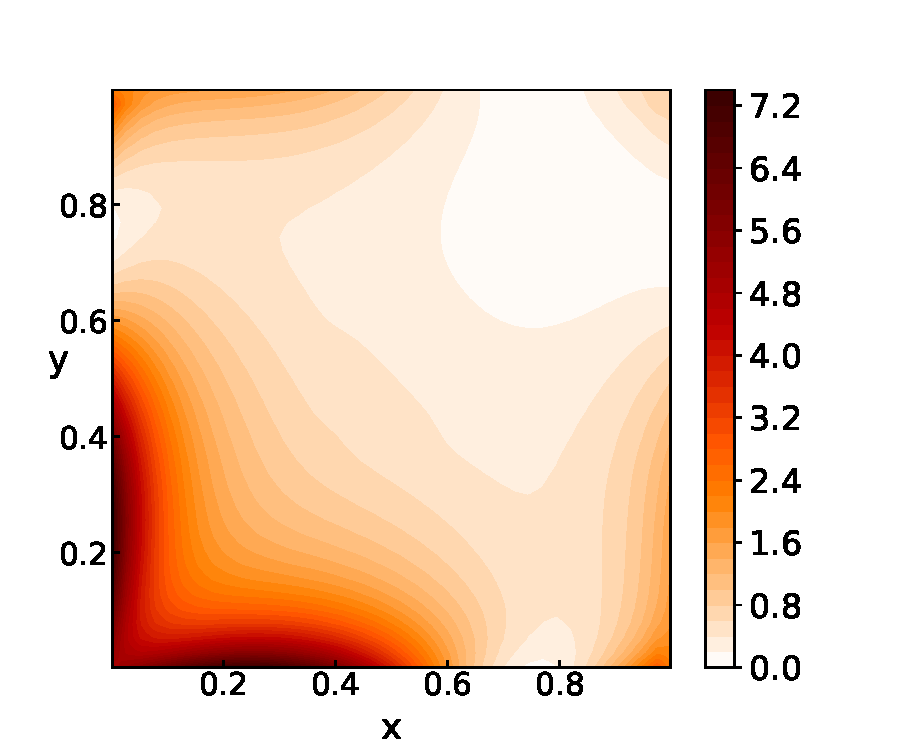
\includegraphics[width=\linewidth]{../../figs/test_g0.99_phi_label.pdf}
		\caption{$\Phi_{\text{label}}$}
		\label{fig:deeprte-g099-label}
	\end{subfigure}\hfill
	\begin{subfigure}[t]{0.32\textwidth}
		\centering
		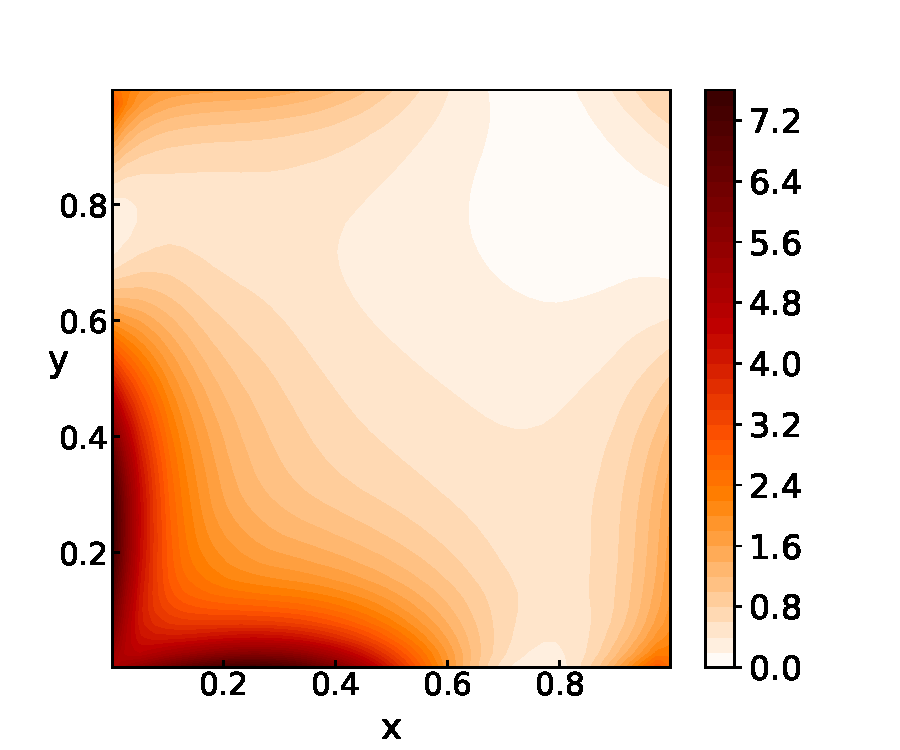
\includegraphics[width=\linewidth]{../../figs/test_g0.99_phi_pre.pdf}
		\caption{$\Phi_{\text{predict}}$}
		\label{fig:deeprte-g099-predict}
	\end{subfigure}\hfill
	\begin{subfigure}[t]{0.32\textwidth}
		\centering
		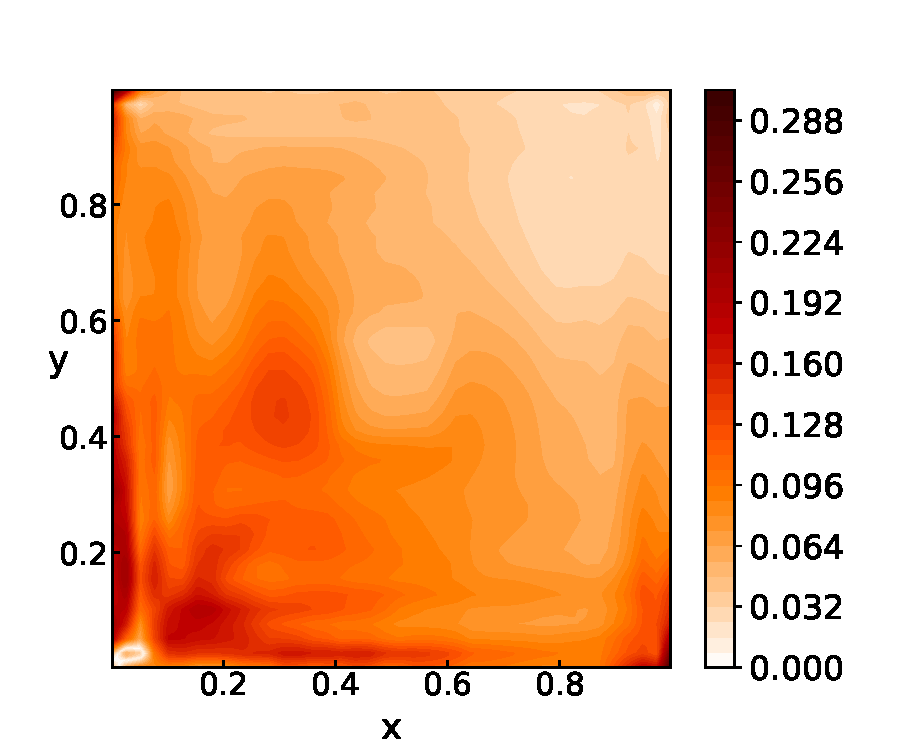
\includegraphics[width=\linewidth]{../../figs/test_g0.99_phi_error.pdf}
		\caption{Absolute error}
		\label{fig:deeprte-g099-error}
	\end{subfigure}
	\caption{DeepRTE evaluation ($g=0.99$).}
	\label{fig:deeprte-g099}
\end{figure}

The figure above illustrates the reference solution $\Phi_{\text{label}}$, the predicted solution $\Phi_{\text{predict}}$, and the absolute error between them. Despite the challenging scenario with $g$ extremely close to 1, DeepRTE demonstrates remarkable accuracy. The quantitative metrics, including an MSE of $0.00764$ and an RMSPE of $4.257\%$, confirm DeepRTE's effectiveness and robustness in handling near-unity anisotropy. This performance highlights DeepRTE's capability to accurately solve the radiative transfer equation even under highly-peaked regime.

\end{reply}

\begin{point}
	Section 6.1: The section is called "mesh independence", but the numerical results and the discussion show that the method (as it is implemented) is actually mesh-dependent in the way that a traditional method is. i think that the section should be renamed into ``mesh dependence'' or ``investigation of mesh dependence''.
\end{point}

\begin{reply}
	Thank you for your suggestion.
	We have rename it to ``Mesh dependence'' as suggested.
\end{reply}

\bibliographystyle{unsrt}
\bibliography{re_refs.bib}

\end{document}
